\chapter{L'editor Medea}                 
\fancyhead[RO]{\bfseries L'editor Medea} 

In questa seconda parte si analizzerà il software Medea realizzato per il progetto. Dapprima verranno illustrati i requisiti funzionali e poi si scenderà nel dettaglio per approfondire la caratteristiche tecniche dell'implementazione data. Alla base ci sono come colonne portanti le tecnologie già ampiamente descritte nella prima parte di questo lavoro. Il compito di questo software è mostrarne potenzialità e limiti.


\section{Prerequisiti}
Per poter utilizzare il software Medea è necessario un browser di ultima generazione che supporti le tecnologie HTML5, WebGL e il relativo Context. Attualmente i layout engines che soddisfano questi requisiti sono Gecko e WebKit vale a dire, elencando solo i browser più popolari che ne fanno uso, Firefox, Chrome e Safari. 
\'{E} inoltre necessario disporre di una scheda grafica e relativi driver che supportino come minimo la specifica OpenGL 2.0 o in alternativa, per gli utenti Windows, l'ultima versione delle DirectX\footnote{Lesson 0: Getting started with WebGL. In \textit{Learning WebGL Blog}. Retrieved 21:00, August 31, 2011, from \url{http://learningwebgl.com/blog/?p=11}}. Va aggiunto che per usufruire agevolmente del software è necessario, soprattutto per quanto riguarda il rendering 3d, che il sistema non rasenti i requisiti minimi, pena una navigazione lenta che costringe spesso al riavvio del browser. Sono caldamente raccomandate schede grafiche ATI e NVidia con gli ultimi driver al seguito, specialmente per sistemi Linux. I driver disponibili per hardware Intel, malgrado supportino WebGL, utilizzano il rendering via software per la visualizzazione delle scene, che risulta accettabile per immagini di piccole dimensioni con pochi oggetti, ma si rivela assolutamente inadatto per visualizzare ambienti complessi con numerosi poligoni.


\section{Strumenti di sviluppo}
L'ambiente di sviluppo è costituito da una macchina su cui gira il sistema operativo GNU/Linux Ubuntu 11.04. La macchina monta una scheda grafica Intel GMA 4500MHD, un hardware che non brilla certo per le sue prestazioni. Proprio per questo è servito anche ad evidenziare quelli che sono i limiti a livello di fruibilità dell'applicazione.

\subsection{Aptana Studio IDE}
Aptana Studio è un Integrated Development Environment opensource improntato allo svillupo di web applications Ajax. Integra già ora il supporto a tecnologie base quali HTML5 e CSS3, DOM e Javascript. Inoltre fornisce gli strumenti per utilizzare importanti framework per applicazioni web quali Ruby on Rails, PHP, Python e Perl. Basato su un solido progetto quale Eclipse, è gratuito e multipiattaforma, ed offre funzionalita di code-completion, code-assist, debugging avanzato e molte altre. 

\begin{figure}[Ht]
\centering
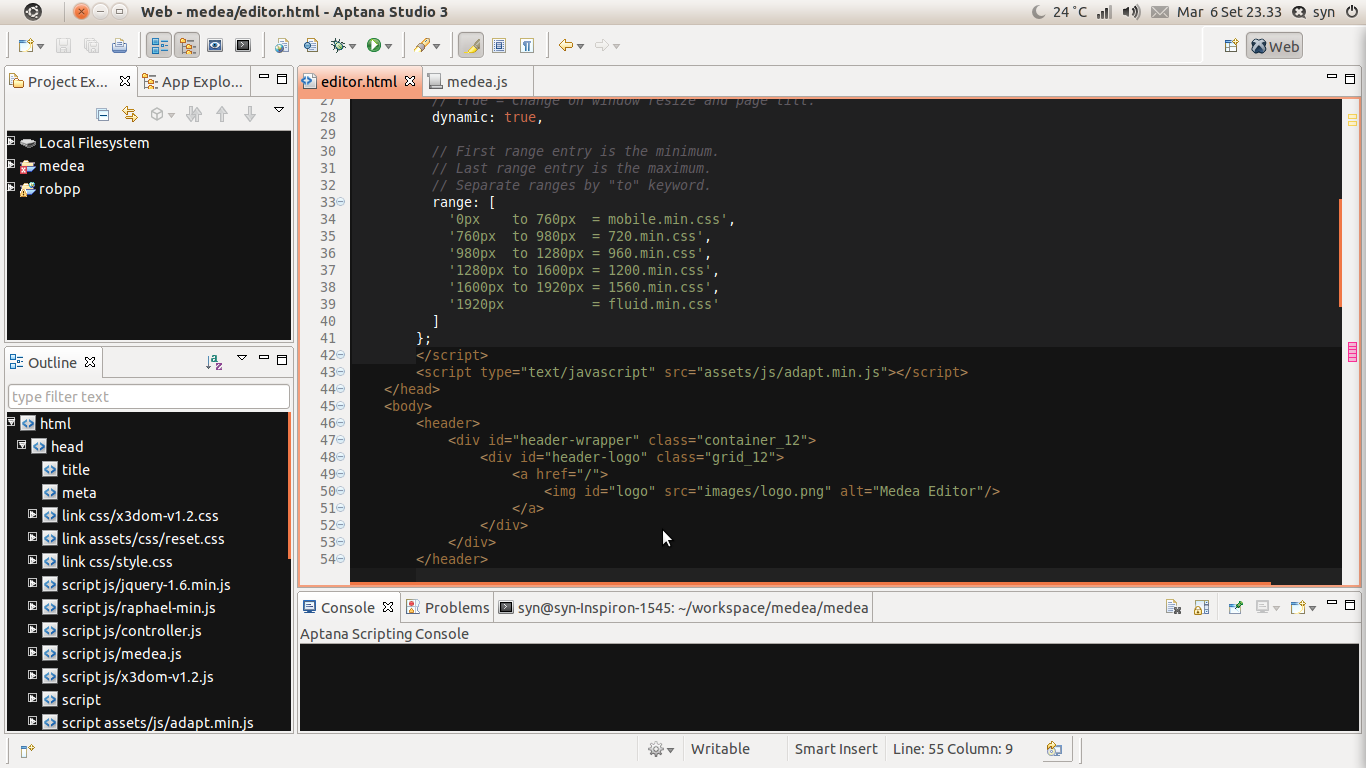
\includegraphics[width=0.9\textwidth]{aptanaui.png}
\caption{Interfaccia di Aptana Studio 3}
\label{label:aptanaui}
\end{figure}

\subsection{Blender per il modeling 3D}
Lo scoglio più grande da superare quando si parla di modellazione 3d è sicuramente quello di trovare un valido tool di supporto a questo difficile compito, in modo particolare se si ha a che fare con oggetti e scene complesse. In questi casi occorre uno strumento che consenta visivamente di modellare le mesh fin nei minimi dettagli. Vi sono molti software proprietari che potrebbero risolvere il problema, ma il prezzo è spesso proibitorio e non sono multipiattaforma. Viene in nostro soccorso Blender, un software per la grafica 3D gratuito, opensource e che supporta a molteplici sistemi operativi.

Nato dalla mente di Ton Roosendal nel 1995 all'interno dello studio di animazione NeoGeo, nel 1998 viene rilasciato come prodotto freeware allo scopo di stimolare interesse da parte degli utenti e quindi offrire servizi di supporto a pagamento. Malgrado l'interesse suscitato e l'enorme community che si era creata intorno, NaN (Not a Number), la società che distribuiva Blender, va in bancarotta nel 2002. Roosendaal però non voleva abbandonare Blender al proprio destino e fonda la “Blender Foundation” con lo scopo di  portarne avanti lo sviluppo. Nel Luglio 2002 parte la campagna “Free Blender”, il cui intento é raccogliere i fondi (100.000\euro) per riacquistare i diritti su Blender e rilasciarlo poi come open source. C'è un'enorme risposta da parte della community e il 13 Ottobre 2002, circa due mesi dopo, l'obiettivo é raggiunto. Blender viene rilasciato con licenza GPL.

Oggi Blender è giunto alla versione 2.59 e già si prepara il terreno per la 2.60. \'{E} un'applicazione completa per la creazione di contenuti 2D e 3D. Contiene tutti gli strumenti di base per il modeling, rendering, lighting, texturing e animazione, oltre a funzionalità avanzate quali un game engine, physic simulation engine e strumenti per la post-produzione. \'{E} estensibile e programmabile grazie ad un motore di scripting Python che ne assicura la massima flessibilità.

Blender integra inoltre un comodo exporter verso numerosi formati, tra cui anche X3D. Questa e le caratteristiche prima citate lo hanno reso strumento indispensabile per la realizzazione di questo progetto.

\begin{figure}[Ht]
\centering
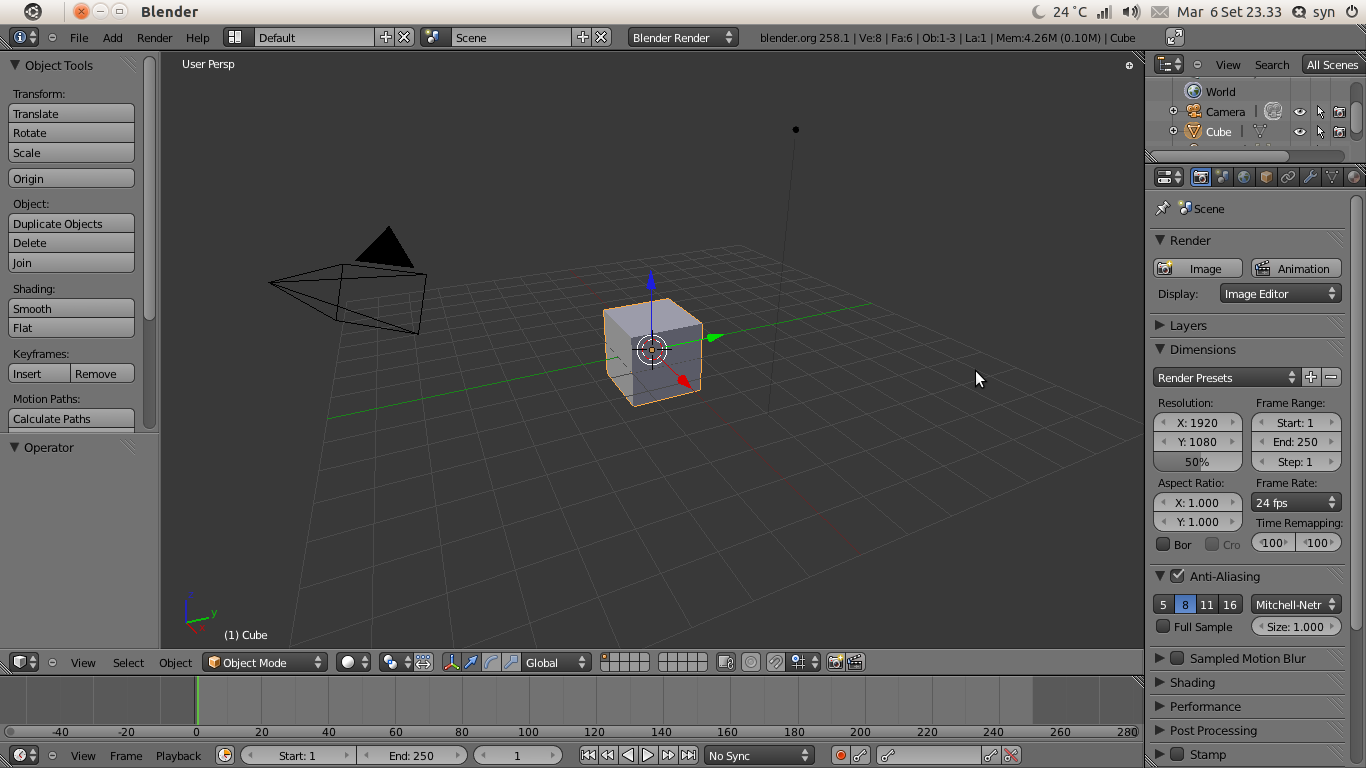
\includegraphics[width=0.9\textwidth]{blenderui.png}
\caption{Interfaccia di Blender}
\label{label:blenderui}
\end{figure}

\subsection{SVG con Raphael JavaScript Library}
Merita di essere citata tra gli strumenti utilizzati anche RaphaelJS. Questa piccola libreria da la possibilità allo sviluppatore di creare attraverso codice Javascript elementi di grafica vettoriale all'interno della pagina web. Alla base c'è lo standard SVG, il markup language per la descrizione di contenuti 2D dichiarativi. Raphael espone dei metodi per il disegno che altro non fanno che creare all'interno del DOM il rispettivo scene-graph SVG (vedi il listato ~\ref{lst:raphael}. Ogni oggetto creato nel DOM è connesso ad un oggetto Javascript e può essere manipolato con facilità, sia grazie agli eventi HTML che da Javascript stesso.

L'obiettivo finale di Raphael, come dice il suo autore Dmitry Baranovskiy, è quello di fornire un libreria per il disegno vettoriale che possa garantire compatibilità cross-browser e al tempo stesso facilità d'uso.

In questo progetto Raphael è stato utilizzato per dar vita ad un controller interattivo che consentisse all'utente di spostare un oggetto all'interno della scena 3d e che fosse allo stesso tempo semplice ed intuitivo. L'intento era anche quello di ``pensionare'' una volta per tutte i tanto abusati slider.

\begin{mylisting}{html}{Esempio di utilizzo della libreria RaphaelJS}{lst:raphael}
// Crea una tela su cui disegnare 400x300 at 10, 10
var paper = Raphael(10, 10, 400, 300);

// Crea un rettangolo di dimensioni 50x50 alle coordinate 25,150
var rect = paper.rect(25, 150, 50,50);
rect.attr("fill", "#f00"); // Lo riempe con il colore rosso
\end{mylisting}

\section{Caso d'uso}
L'idea alla base di questo progetto è quella di fornire all'utente un'ambiente che gli consenta di navigare in un mondo virtuale, con la possibilità di collocarvi degli oggetti a piacere. Le scene a disposizione e gli oggetti faranno parte di una libreria che verrà creata in base alle specifiche esigenze. L'obiettivo del progetto è difatti quello di sviluppare la struttura che consenta di contenere le scene e di inserire e muovere gli oggetti, e non quello di disegnare gli oggetti stessi. Va da se che un caso concreto è stato comunque creato. Come ambiente di prova è stato modellato un minimarket e alcuni dei relativi prodotti. Nelle figure ~\ref{label:marketbrout} e ~\ref{label:marketbrin} si possono vedere due rendering dell'ambiente creato, effettuati con blender.

\begin{figure}[Ht]
\centering
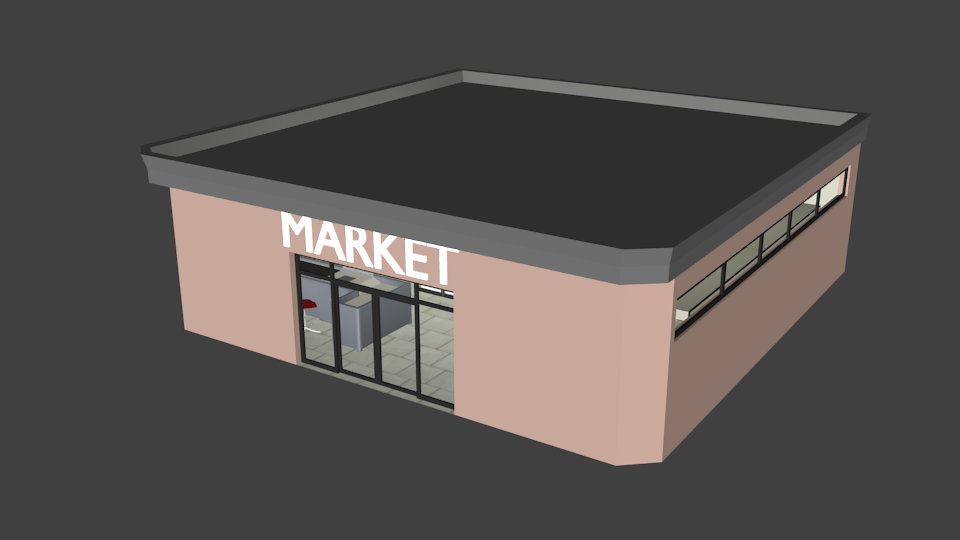
\includegraphics[width=0.7\textwidth]{marketbrout.png}
\caption{Market rendering: esterno}
\label{label:marketbrout}
\end{figure}

\begin{figure}[Ht]
\centering
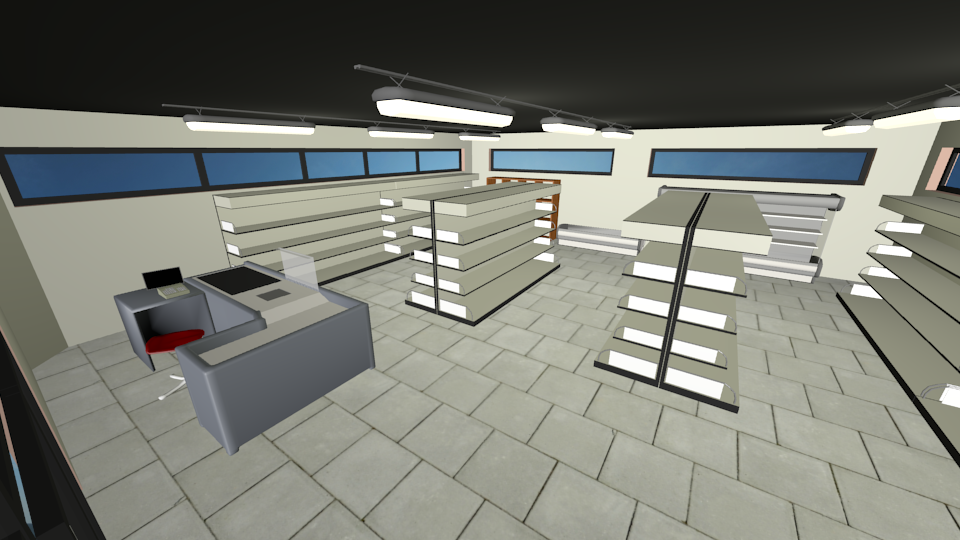
\includegraphics[width=0.7\textwidth]{marketbrin.png}
\caption{Market rendering: interno}
\label{label:marketbrin}
\end{figure}

L'interfaccia, come già anticipato, sarà il browser e tutti i contenuti dovranno essere fruibili direttamente dalla pagina web, che si comporrà di tre componenti fondamentali: il canvas per la scena 3d, un controller per la navigazione, lo spostamento, rotazione e rimozione degli oggetti, e la lista degli oggetti presenti in libreria da poter inserire nella scena. Infine serve un motore che faccia da collante e tenga insieme il tutto. In Figura ~\ref{label:mockupui} si può vedere una bozza dell'interfaccia utente finale. Non tutte le features presentate saranno implementate in questo progetto. 

Quest'interfaccia mira ad essere semplice ed immediata per l'utente, operando alcune scelte fondamentali:
\begin{itemize}
    \item Utilizzo del Drag 'n Drop HTML5 per l'inserimento degli oggetti di libreria nella scena;
    \item Controller SVG semplificato ed intuitivo in sostituzione dei classici slider;
\end{itemize}

\begin{figure}[Ht]
\centering
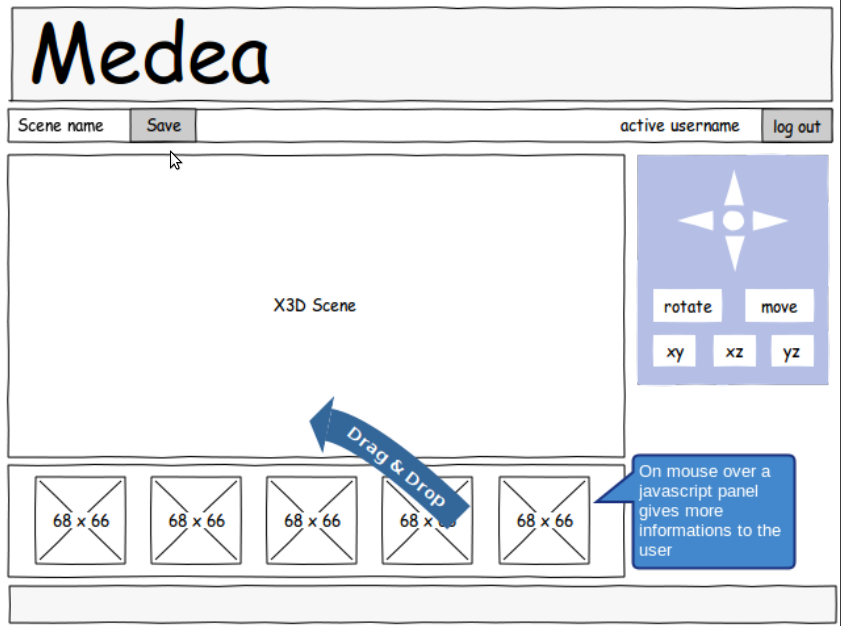
\includegraphics[width=0.8\textwidth]{mockupui.png}
\caption{Medea User Interface}
\label{label:mockupui}
\end{figure}
%\clearpage

\section{Le caratteristiche tecniche}

\subsection{La struttura}
Medea si divide in due parti: client e server. La parte client è tenuta insieme da un motore javascript che si occupa dell'interazione utente in tutti i suoi aspetti. Dalla creazione del controller, alla gestione del darg 'n drop e della posizione degli oggetti nella scena. Il lato server è mantenuto estremamente semplice e al momento si preoccupa solo di caricare dinamicamente la libreria degli oggetti.

Per una maggiore chiarezza della struttura del progetto, di seguito viene mostrata l'organizzazione nel filesystem con le componenti principali in evidenza:

\begin{mylisting}{sh}{Struttura filesystem medea}{lst:medeafs}
medea
|-- app.py              # Applicazione server
|-- config.py           # Modulo di configurazione server
|-- static              # File statici
|   |-- assets
|   |-- css
|   |-- images
|   |-- js
|   o-- x3d
|       |-- library     # Libreria oggetti
|       |-- market      # Scena minimarket
|       o-- textures
|-- templates           # Template html utilizzati
|   o-- editor.html     
o-- view.py             # Modulo di rendering dei template html
\end{mylisting}


\subsection{Il server: Webpy framework}
Alla base del software Medea c'è Webpy, un framework Python per creare web-application dinamiche. Webpy ci consente di creare un mapping tra url e oggetti python, che serviranno le richieste fatte dal client. Il codice server creato è semplice e di immediata comprensione. 

\begin{mylisting}{python}{Medea server}{lst:medeaserver}
import web, os
import config
from view import render

urls = ('/', 'editor',)

application = web.application(urls, globals())

class editor(object):
    def GET(self):
        lib = parse_library(config.LIBRARY_PATH)
        return render.editor(lib)

def parse_library(path):
    import fnmatch
    files = map(lambda x: os.path.join(path,x), os.listdir(path)) 
    
    inlines = sorted(fnmatch.filter(files, "*.x3d"))
    thumbs = sorted(fnmatch.filter(files, "*.png"))

    return zip(inlines, thumbs)
\end{mylisting}

Il modulo python \texttt{web} è il cuore del framework e ci consente di creare l'oggetto \texttt{application} che si occuperà di servire le richieste, secondo il mapping definito a linea 6. In questo caso la mappatura è elementare: sono consentite solo richieste indirizzate alla 'root' e queste vengono servite da un'istanza della classe \texttt{editor}, la quale definisce un comportamento per il solo metodo HTTP GET.

Questo metodo carica tutti i file di libreria, collocata in un path specificato nel modulo di configurazione, chiamando la funzione \texttt{parse-library}. Dopodich\'{e} renderizza il template \texttt{editor.html} passandogli come parametro la lista ottenuta e restituisce il risultato al client. Il listato ~\ref{lst:library} mostra un estratto del template, in particolare la parte in cui viene creata la libreria. Il motore di templating utilizza il carattere '\$' come escape per includere codice python all'interno della pagina html. Quando il template viene processato il codice incluso viene riconosciuto ed eseguito per generare la pagina dinamicamente. \'{E} possibile passare al template dei parametri in input. In questo caso viene fornita la lista degli oggetti in libreria. Ogni oggetto contiene l'url del file x3d e dell'immagine. Il ciclo \texttt{\$for x3d, thumb in library} produce un elemento \texttt{<li>} con questi dati.

\begin{mylisting}{html}{Medea: template libreria}{lst:library}        
<div id="library" class="grid_12">
        $if library:
            <ul>
            $for x3d, thumb in library:        
                <li>
                    <div class="grid_1 draggable">
                        <img src="$thumb" width="50px"></img>
                        <inline url="$x3d"></inline>
                    </div>
                </li>
            </ul>
        $else: 
            <p><big>Your library is empty!</big><p>
</div>
\end{mylisting}


\subsection{Il client: medea.js}
Lato client il motore \texttt{medea.js} si occupa di inizializzare i componenti che compongono l'interfaccia, connettendo gli eventi ai rispettivi metodi di gestione. Nel codice si fa uso della libreria jQuery per rendere la sintassi meno prolissa e più chiara.

\begin{mylisting}{Java}{Medea client}{lst:medeajs1}
// Loading controller
var controller = Raphael.controller(0, 0, 200, "controller");
var medea = {};
medea.range = 2; // This defines the sensibility of the controller 
medea.step = 0.785; // Rotation step
medea.plane = null;
medea.selected = null;
medea.select = function () {
    var highlight = '<shape class="highlight"><sphere radius="0.2"/><appearance><material diffuseColor="1 0 0" transparency=".9"/></appearance></shape>';
    
    return function (ev) {
        console.log(ev.target);
        $(".highlight").remove();
        
        if (ev.target === medea.selected) {
            medea.selected = null;
        } else {
            medea.selected = ev.target;
            $(ev.target).append(highlight);
        }
    };
}();
medea.remove = function () {
    if (!medea.selected) return;
    
    $(medea.selected).remove();
    $(".highlight").remove();
}
$("#x3d_element transform.selectable").click(medea.select);
$("#remove_bt").click(medea.remove);
\end{mylisting}

\texttt{medea.js} è eseguito alla fine del caricamento della pagina. Il primo ad essere creato è il controller, del quale saranno dati i dettagli implementativi più avanti. Il metodo \texttt{Raphael.controller} prende in input la posizione (coordinate x, y), la dimensione e l'id dell'elemento HTML nel quale disegnare il controller. Vengono poi inizializzati alcuni parametri che specificano la sensibilità del controller durante il movimento, il piano su cui l'oggetto si muove e lo step di rotazione degli oggetti in radianti. La rotazione è stata vincolata sul solo asse y a step di 45 gradi per facilitare l'utente nel posizionamento. Segue la funzione \texttt{medea.select} che gestisce il click sull'oggetto della scena 3d marcandolo come selezionato, sia internamente, valorizzando la variabile di stato \texttt{medea.selected} con il rispettivo oggetto javascript, sia visivamente per l'utente, aggiungendo una sfera semitrasparente intorno all'oggetto. Nelle ultime due istruzioni le funzioni sopra descritte vengno connesse agli eventi degli elementi che li gestiscono. Da notare che per la selezione la funzione \texttt{medea.select} viene agganciata ai soli nodi transform che abbiano classe \texttt{selectable}, così da impedire all'utente di spostare qualsiasi mesh presente nell'ambiente.

L'inserimento viene gestito grazie al Drag'n Drop che HTML5 implementa nativamente. Nella pratica, ogni elemento che abbia l'attributo \texttt{draggable} impostato a \texttt{true} è trascinabile. Di seguito il codice che gestisce questa funzionalità.

\begin{mylisting}{Java}{Medea client: il Drag'n Drop}{lst:medeajs2}
//Indica al browser quali elementi sono trascinabili, in questo caso attraverso una classe.
$(".draggable").attr("draggable", "true")
//Specifica cosa fare quanto un elemento viene trascinato
.bind('dragstart', function(ev) {
    var dt = ev.originalEvent.dataTransfer;
    var html = $('<div>').append($(this).find("inline").clone()).remove().html();
    dt.setData("node", html);
    return true;
});

//Indica al browser l'elemento in cui puoi trascinare gli oggetti.
$("#drop").bind("dragenter", function (ev) {
    return false;
}).bind("dragleave", function (ev) {
    return false;
}).bind('dragover', function(ev) {
    return false;
}).bind("drop", function (ev) {
    //con questa riga ottengo i dati salvati quando ho iniziato a trascinare l'oggetto'
    var tmp = ev.originalEvent.dataTransfer;
    var node = $(medea.transform).append(tmp.getData("node"));
    
    $(this).find("scene").append(node);

    // Binding click event to selection function
    $(this).find("scene transform.selectable:last").click(medea.select);
    return false;
});
\end{mylisting}

Il codice può sembrare di difficile comprensione; in realtà la parte interessante è nelle due funzioni che gestiscono gli eventi ``dragstart'' e ``drop''. La prima specifica le azioni da intraprendere quando inizia un'azione di trascinamento. In questo caso viene memorizzato il contenuto html dell'elemento trascinato nell'oggetto \texttt{dataTransfer}\footnote{L'oggetto dataTransfer può essere visto come un'area di comunicazione condivisa disponibile solo se si verifica uno degli eventi legati al drag'n drop} con la chiave "node". Nel contenuto html dell'elemento ``draggable'' è stato preventivamente predisposto dal server il tag \texttt{<inline>} che fa riferimento all'oggetto. La funzione legata al ``drop'' a questo punto non fa altro che recuperare il contenuto del \texttt{dataTransfer} con la stessa chiave, lo inserisce in un un nodo \texttt{<transform>} selezionabile e lo incorpora nella scena X3D.

Ultime funzioni degne di nota sono \texttt{medea.rotate} e \texttt{medea.moving} nel listato ~\ref{lst:medeajs3}. La prima manipola l'attributo \texttt{rotation} del nodo selezionato e viene banalmente agganciata al click dei pulsanti con id ``rleft'' e ``rright''. La seconda, più interessante, calcola la posizione dell'elemento selezionato sulla base dei due parametri in input \texttt{vu} e \texttt{vv}. La funzione si aspetta che questi valori siano compresi tra 0 e 1 per essere poi moltiplicati per la variabile \texttt{medea.range}, che ne definisce dunque la sensibilità. \texttt{medea.moving} viene passata come funzione di ``callback'' al controller, il quale, ad ogni variazione, la richiamerà impostando opportunamente i due valori richiesti in input.

\begin{mylisting}{Java}{Medea client: movimento e rotazione}{lst:medeajs3}
medea.rotate = function (clockwise) {
    if (!medea.selected) return;
    
    var r = medea.getRotation($(medea.selected).attr('rotation'));
    r.y = 1;
    
    r.g += clockwise ? -medea.step : medea.step;
    $(medea.selected).attr('rotation', r.x +" "+ r.y +" "+ r.z +" "+ r.g);
}
$("#rleft").click(function (ev) {
    medea.rotate(true);
});
$("#rright").click(function (ev) {
    medea.rotate(false);
});
    
medea.moving = function (vu, vv) {
    if (!medea.selected) return;
    var pos = medea.getPos($(medea.selected).attr('translation'));
    
    pos[medea.plane[0]] += vu*medea.range;
    pos[medea.plane[1]] += vv*medea.range;            
    $(medea.selected).attr('translation', pos.x +" "+ pos.y +" "+ pos.z);
}

controller.bind(medea.moving);
\end{mylisting}

\subsection{Il controller}
Il componente \texttt{controller.js} ha il compito di disegnare il controller SVG per il movimento degli oggetti. Grazie alla libreria RaphaelJS, questo compito può essere svolto interamente dal codice javascript.

Quello che si è cercato di fare è creare un elemento che estende le funzionalità della libreria Raphael con un nuovo componente, istanziabile grazie al metodo \texttt{Raphael.controller}. L'oggetto Controller è stato reso indipendente dal progetto Medea ed è quindi sganciabile e riutilizzabile.

\begin{mylisting}{Java}{Medea client: il controller SVG}{lst:controllerjs1}
(function (Raphael) {
    Raphael.controller = function (x, y, size, element) {
        return new Controller(x, y, size, element);
    };
    
    var Controller = function (x, y, size, element) {
        // *** start drawing controller
        size = size || 200;
        var size2 = size / 2,
            size5 = size / 5,
            size10 = size / 10;
            padding = size * 0.02,
            width = size * 0.02;
        
        var r = element ? Raphael(element, size, size) : Raphael(x, y, size, size);
        
        // Controller area
        // [... code omitted ...]
        
        // Events
        // Cursor drag
        var t = this; 
        t.cursor.drag(
            function (dx, dy) {
                this.attr({
                    cx: Math.min(Math.max(this.ox + dx, lbound), rbound),
                    cy: Math.min(Math.max(this.oy + dy, lbound), rbound)
                })
                
                if (typeof t._movecback === 'function') {
                    var vx = (dx / this.ox) - (this.odx / this.ox),
                        vy = (-dy / this.oy) - (this.ody / this.oy);
                     
                    t._movecback(vx, vy);
                    this.odx = dx, this.ody = -dy;
                }
            },
            function () {
                this.ox = this.attr("cx");
                this.oy = this.attr("cy");
                
                this.odx = 0;
                this.ody = 0;
                
                if (typeof t._startcback === 'function') t._startcback();
            },
            function () {
                this.stop();
                this.attr({cx: this.ox, cy: this.oy, opacity: 1});
                
                if (typeof t._stopcback === 'function') t._stopcback();
            }
        );
    };
    
    // Binding callback functions
    Controller.prototype.bind = function (move, start, stop) {
        if (typeof move === 'function') this._movecback = move;
            
        if (typeof start === 'function') this._startcback = start;
           
        if (typeof stop === 'function') this._stopcback = stop;
    };
})(window.Raphael);
\end{mylisting}

Il listato ~\ref{lst:controllerjs1} mostra la crezione dell'area di controllo, tralasciando la parte di disegno, specifica della libreria Raphael. Vengono invece riportate i metodi che gestiscono il trascinamento del cursore per mostrare come sono state agganciate le callback. Oltre alla funzione \texttt{movecback} è stata prevista la possibilità di fornire, sempre tramite il metodo \texttt{Controller.bind}, due funzioni per gli eventi di ``dragstart'' e ``dragstop''.

\subsection{L'interfaccia finale}
Non resta altro che mettere insieme i pezzi del puzzle. Con poche righe di codice, si carica il motore x3dom.js, responsabile dell'integrazione e del rendering della scena X3D. Al caricamento della pagina, X3DOM verifica la presenza di un tag \texttt{<x3d>} nel DOM della pagina e, qualora fosse presente, aggiunge un elemento \texttt{canvas} per la visualizzazione della scena tramite WebGL. Nel listato ~\ref{lst:editorx3d} la scena x3d è inclusa direttamente nella pagina. Ciò non toglie che sarebbe auspicabile una funzione lato server che la carichi dinamicamente all'interno di un \texttt{<div>} predefinito, similmente a quanto fatto per la gestione della libreria.

\begin{mylisting}{html}{Medea: editor.html}{lst:editorx3d}
<!DOCTYPE html>
<html>
    <head>
        <title>Medea Scene Editor</title>
        <!-- x3dom -->
        <link rel='stylesheet' type='text/css' href='http://www.x3dom.org/x3dom/release/x3dom.css'></link>
        <script type='text/javascript' src='http://www.x3dom.org/x3dom/release/x3dom.js'></script>

        <script type="text/javascript" src="/static/js/controller.js"></script>
        <script type="text/javascript" src="/static/js/medea.js"></script>        
    </head>
    <body>
        <!-- [ ... code omitted ...] -->        
        
        <div id="drop" class="grid_9">
            <x3d id='x3d_element' showStat='false' showLog='false' x='0px' y='0px' width='880px' height='400px'>
                <scene id="root_scene">
                    <background skyColor='0 0 0'></background>
                    <navigationinfo headlight="true" type="EXAMINE" avatarSize="0.25, 0.75, 0.75"></navigationinfo>
                    <viewpoint DEF='FrontView' description='Front View' position='0.01 0.80 2.80'></viewpoint>
                    <inline url="x3d/market/minimarket_out.x3d"></inline>
                </scene>
            </x3d> 
        </div>
\end{mylisting}

La Figura ~\ref{label:medeaui01} mostra l'interfaccia utente finale del software Medea, mentre in Figura ~\ref{label:medeaui02} è immortalato un utente in fase di posizionamento dell'oggetto selezionato.
\clearpage

\begin{figure}[Ht]
\centering
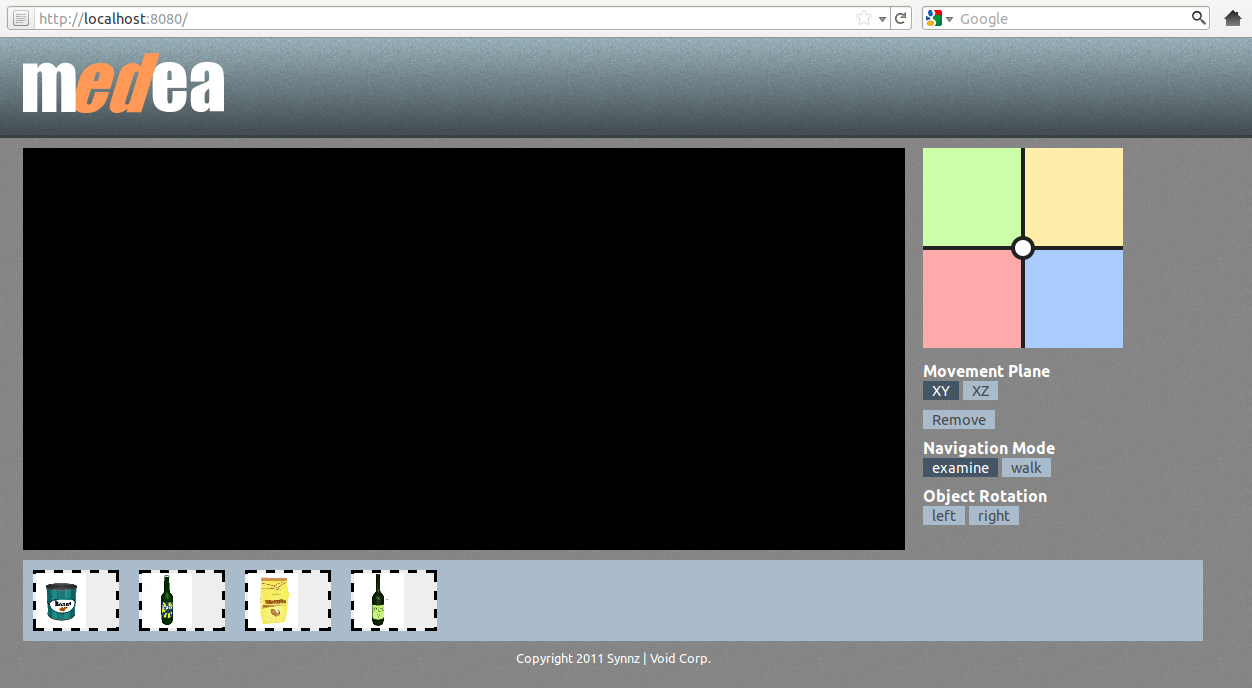
\includegraphics[width=0.9\textwidth]{medeaui01.png}
\caption{Interfaccia utente finale}
\label{label:medeaui01}
\end{figure}

\begin{figure}[Ht]
\centering
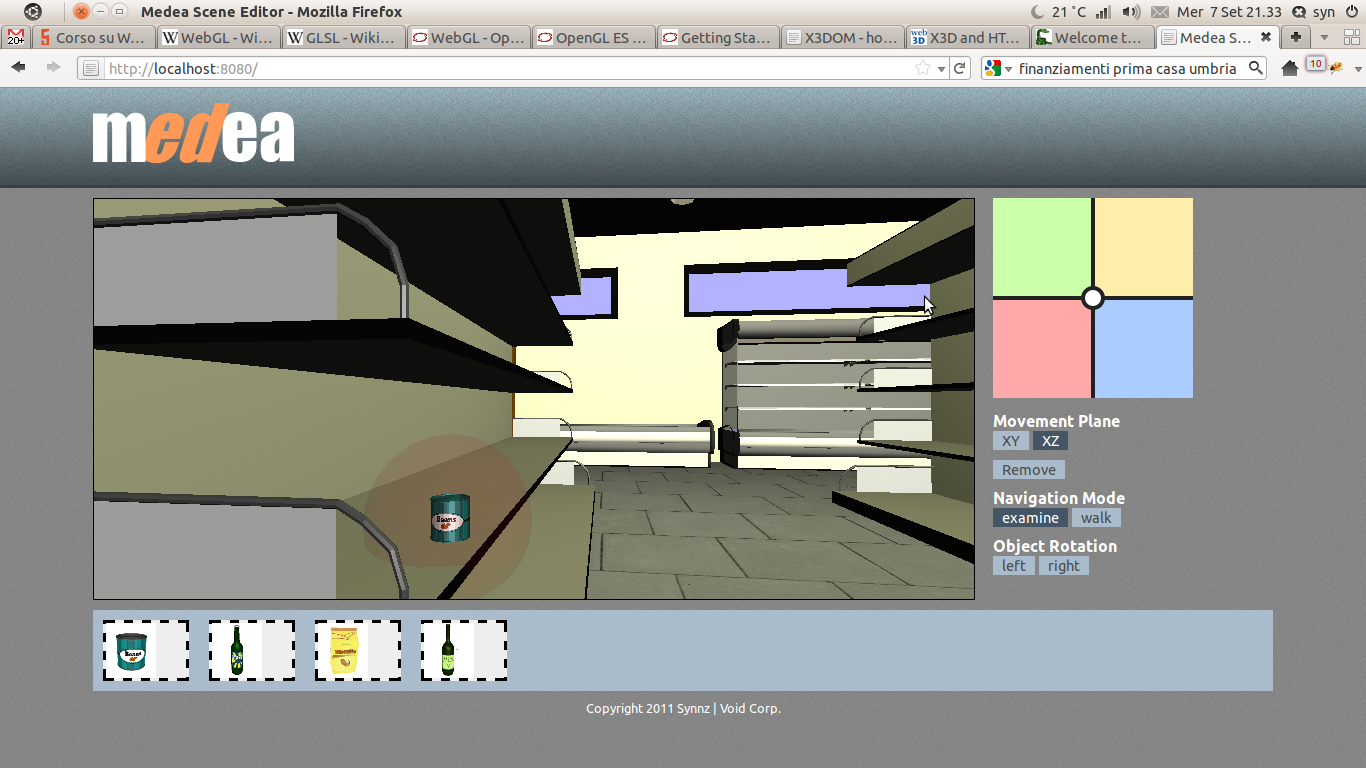
\includegraphics[width=0.9\textwidth]{medeaui02.png}
\caption{Utente durante il posizionamento di un oggetto selezionato}
\label{label:medeaui02}
\end{figure}


